\chapter{Introduction} 

	\setcounter{section}{1}
\section{Concepts et définitions}
	\subsection{Système thermodynamique et volume de contrôle}
	La première chose à savoir est qu'il faut définir la \textit{frontière 
	du système}, délimitant un \textit{volume de contrôle}. Tout l'au delà 
	de la frontière est le \textit{milieu extérieur}.\\
	
	La frontière défini des types de systèmes
	\begin{enumerate}
	\item \textbf{Fermé} : Si la frontière est imperméable (la matière ne 
	peut la traverser)
	\item \textbf{Isolé} : Si la frontière est imperméable et s'il n'y a 
	aucun échange avec le milieu extérieur.
	\item \textbf{Ouvert} : Si la frontière est traversée par un débit de 
	masse.
	\end{enumerate}
	
	\begin{wrapfigure}[6]{l}{7cm}
	\vspace{-6mm}
	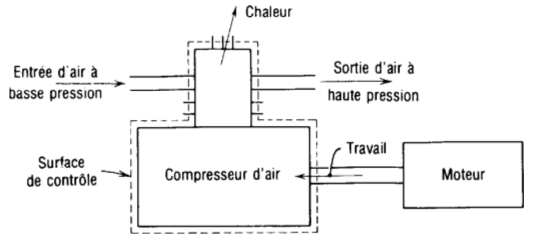
\includegraphics[scale=0.3]{ch1/image1.png}
	\captionof{figure}{ }
	\end{wrapfigure}
	Par exemple, l'image ci-contre est un système ouvert car l'air 
	rentre et sort (par les \textit{sections d'entrée et de sortie}) (même 
	si tout le système n'est pas traversé). On remarque que la frontière 
	traverse ici l'arbre du moteur (pas d'échange de chaleur , mais 
	d'énergie).
	
	
	\subsection{Points de vue macroscopique et microscopique}
	Nous allons utiliser le point de vue macroscopique en ne s'intéressant  
	qu'aux manifestations globales de l'ensemble des atomes. L'intérêt du 
	macro est que l'on peut caractériser un système avec des senseurs (
	thermomètre, \dots). Pour adopter ce point de vue, il est nécessaire 
	de travailler avec un "grand" nombre de molécules ($\approx 10^9$ atomes 
	de gaz tiennent dans $10^{-11}$ cm$^3$). Dans ces conditions, on peut 
	décrire la matière comme un \textit{milieu continu} : si on choisi un 
	point et que que l'on se déplace, $p$ et $T$ vont varier de façon 
	continue.
	
	\subsection{Variables et états d'une substance}
	La matière peut se présenter selon différents \textit{états}. Cet 
	état thermodynamique est caractérisé par des \textit{variables d'état} 
	dont la valeur ne dépend que de l'état de la substance. Elles peuvent 
	être
	\begin{itemize}
	\item[$\bullet$] \textbf{Intensives} ; peuvent se définir en tout point 
	d'un système $(p, T)$.
	\item[$\bullet$] \textbf{Extensives} ; ne sont définies que pour un 
	système dans son entièreté ($m, V$).
	\end{itemize}
	On peut faire correspondre à une variable extensive une variable intensive 
	massique, volumique ou encore molaire.\\
	Un système uniforme est dit en \textit{équilibre} si les variables 
	restent constantes dans le temps.
	
	
	\subsection{Transformations et cycles}
	Lorsque les variables d'état sont modifiées, le système subit un \textit{
	changement d'état}. La succession d'état est une \textit{transformation} 
	du système. \\
	
	\begin{wrapfigure}[7]{r}{4.7cm}
	\vspace{-7mm}
	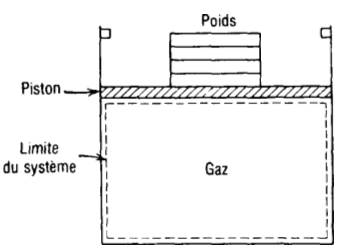
\includegraphics[scale=0.4]{ch1/image2.png}
	\captionof{figure}{ }
	\end{wrapfigure}
	Considérons l'exemple du poids sur le piston. Le système est 
	en équilibre (mécanique). Si l'évolution est suffisament lente, on peut 
	considérer que le système est en équilibre, les écarts entre l'équilibre 
	et l'état intermédiaire étant infinitésimaux. Ces états sont en 
	\textit{quasi-équilibre}. Si hélas l'échange est trop rapide, lah la 
	thermo est impuissante à décrire les états intermédiaires.\\
	Notons que si une variable d'état reste constante, on la dénote par le 
	préfixe "iso".\\
	
	Si au cours d'une transformation, le système retrouve son état initial en 
	passant par une succession d'états intermédiaires distincts on parle de 
	\textit{cycle}. Si l'état final diffère de l'initial, on parle de \textit{
	transformation ouverte}.
	
	
	\subsection{Le volume massique}
	Si le système est uniforme, on note le volume massique 
	\begin{equation}
	v = \frac{V}{m}
	\end{equation}
	Si le système est non-uniforme, le volume en un point $P$ est défini 
	par
	\begin{equation}
	v = \lim\limits_{\delta V \rightarrow \delta V'} \frac{\delta V}{
	\delta m}
	\end{equation}
	où $\delta m$ est la masse contenue dans le volume $\delta V$ autour 
	de $P$. On tend vers $\delta V'$ et non vers zéro afin de garder nos 
	$10^9$ éléments et rester dans le cadre d'une vue macroscopique.
	
	Le volume molaire\footnote{Les grandeurs molaires sont surmontée d'un 
	tiret.} est quant à lui défini par
	\begin{equation}
	\overline{v} = \lim\limits_{\delta V \rightarrow \delta V'} \frac{
	\delta V}{\delta n}
	\end{equation}
	où $\delta n$ est le nombre de moles contenue dans $\delta V$. La 
	masse volumique, $\rho$, est l'inverse du volume massique.
	
	
	\subsection{La pression}
	Soit $P$, situé sur la surface $S$ d'un volume contenant un fluide, 
	$\delta \vec F$ la force exercée sur un élement de surface d'aire 
	$\Delta \mathcal{A}$. Si le fluide est en repos, cette force est 
	normale et la pression $p$ du fluide est définie par
	\begin{equation}
	p = \lim\limits_{\delta\mathcal{A}\rightarrow\delta\mathcal{A}'} 
	\frac{\delta F}{\delta \mathcal{A}}
	\end{equation}		
	Dans un fluide visqueux en mouvement, la force de surface n'est 
	plus que normale. Néamoins dans ce cours on négligera les effets 
	de viscosités et tous les fluides seront parfaits.\\
	Notons qu'on considère toujours la pression absolue (par rapport 
	au vide). Attention donc aux pressions relatives qui prennent 
	généralement $P_{atm}$ comme référence : il ne faut pas oublier 
	d'ajouter cette pression de référence à la pression indiquée 
	pour les calculs !
	
	
	\subsection{Égalité des températures}
	Deux corps en contacts à températures différentes vont subir une 
	variation de leurs propriétés observables (dimension, résistance 
	électrique, indice de réfraction) jusqu'à atteindre l'\textit{
	équilibre thermique}.
	
	\subsection{Le principe zéro de la thérmodynamique}
	Il s'agit d'un postulat non démontrable par A. Sommerfeld (1956). 
	Deux corps en équilibre thermique avec un troisième sont aussi 
	en équilibre thermique entre eux.
	
	\subsection{Les échelles de température}
	Le plus simple est de travailler avec des points fixe comme pour 
	l'eau (0$^\circ$ et 100$^\circ$). Il est parfois possible de 
	définir une échelle de température indépendantes des propriétés 
	d'un thermomètre : on parlera d'\textit{échelle de température 
	thermodynamique.}
	
	
	
	
	
	
	
	
	
	
	
	
	
	
	
	
	
	
	
	
	
	
	
	
	
	
	
	
